\documentclass{standalone}
\usepackage{amsmath}
\usepackage{amssymb}
\usepackage{warpcol}
\usepackage{array}
\usepackage{esint}
\usepackage{subfig}
\usepackage{rotating}
\usepackage{booktabs}
\usepackage{paralist}
\usepackage{graphicx}
\usepackage{physics}
\usepackage{ucs}
\usepackage{indentfirst}
\usepackage{tikz}
\usepackage{colortbl}
\usepackage{xcolor}
\usepackage{xeCJK}
    \setCJKmainfont[BoldFont={Noto Serif CJK SC Bold},ItalicFont={FangSong}]{Noto Serif CJK SC}
    \setCJKsansfont[BoldFont={Noto Sans CJK SC Bold},ItalicFont={KaiTi}]{Noto Sans CJK SC}
    \setCJKmonofont[BoldFont={Noto Sans Mono CJK SC Bold}]{Noto Sans Mono CJK SC}

\DeclareUnicodeCharacter{"00B0}{\textdegree}
\DeclareUnicodeCharacter{"2103}{\textcelsius}

\pgfsetxvec{\pgfpoint{2.5em}{0}}
\pgfsetyvec{\pgfpoint{0}{2.5em}}

\usetikzlibrary{angles,patterns,datavisualization,plotmarks,arrows.meta,datavisualization.formats.functions,decorations.markings}

\newcommand{\hexagon}[2]{
    \draw[line cap=round] (#1,#2) -- (#1+1,#2-0.5) -- (#1+1,#2-1.5) -- (#1,#2-1) -- (#1,#2);
}
\newcommand{\anohexagon}[2]{
    \draw[line cap=round] (#1,#2) -- (#1+1,#2-0.5) -- (#1+1,#2-1) -- (#1,#2-1.5) -- (#1,#2);
}

\begin{document}
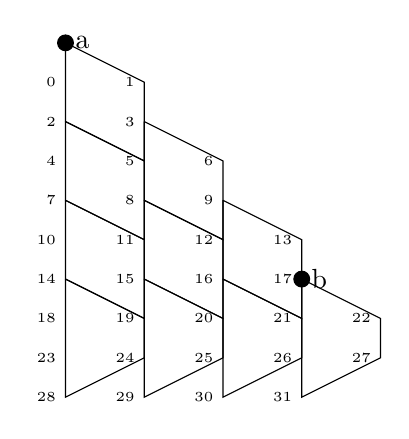
\begin{tikzpicture}
\foreach \x/\y in {
    0/0,
    0/-1, 1/-1,
    0/-2, 1/-2, 2/-2
}{
    \hexagon{\x}{\y}
}
\foreach \x/\y in {
    0/-3, 1/-3, 2/-3, 3/-3
}{
    \anohexagon{\x}{\y}
}
\foreach \x/\y[count=\idx] in {
    0/-.5, 1/-.5,
    0/-1, 1/-1,
    0/-1.5, 1/-1.5, 2/-1.5,
    0/-2, 1/-2, 2/-2,
    0/-2.5, 1/-2.5, 2/-2.5, 3/-2.5,
    0/-3, 1/-3, 2/-3, 3/-3,
    0/-3.5, 1/-3.5, 2/-3.5, 3/-3.5, 4/-3.5,
    0/-4, 1/-4, 2/-4, 3/-4, 4/-4,
    0/-4.5, 1/-4.5, 2/-4.5, 3/-4.5
}{
    \node[left] at (\x, \y) {\tiny\pgfmathparse{int(\idx-1)}\pgfmathresult};
}
\filldraw (0, 0) node[right] {a} circle (0.1);
\filldraw (3, -3) node[right] {b} circle (0.1);
\end{tikzpicture}
\end{document}
